\documentclass[12pt,a4paper]{article}
\usepackage[utf8]{inputenc}
\usepackage{graphicx}
\usepackage{geometry}
\usepackage{enumitem}
\usepackage{titlesec}
\usepackage{hyperref}

\geometry{margin=2.5cm}

\title{Regional and Seasonal Comparative Analysis}
\date{}

\begin{document}

\maketitle

\section*{1. Trend of Student Count in Each Region by Season}
Figure~\ref{fig:student-count-region-season} illustrates how the number of students from each region varied across seasons. Shiraz consistently dominates in all seasons, peaking in Summer (nearly 59 students). Fars shows a gradual increase from Winter (about 12 students) to Summer (about 22), then a slight decline in Autumn. Other regions remain relatively stable with smaller student numbers, though "Unknown" and Bushehr show some upward movement by Autumn. This trend suggests higher demand for courses in Summer, particularly in central regions.

\begin{figure}[h!]
    \centering
    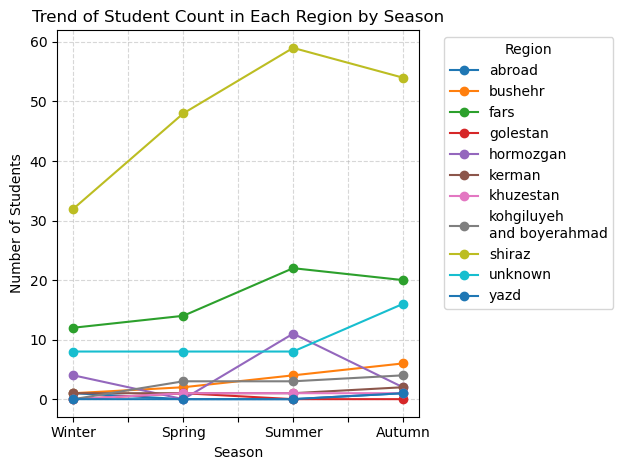
\includegraphics[width=1\textwidth]{Trend of Student Count in Each Region by Season.png}
    \caption{Trend of Student Count in Each Region by Season}
    \label{fig:student-count-region-season}
\end{figure}

\section*{2. Income Trend in Each Region by Season}
Figure~\ref{fig:income-region-season} shows how the total income from each region fluctuated seasonally. Shiraz again leads, reaching over 3.4 billion IRR in Summer, then slightly dropping in Autumn. Fars and "Unknown" regions also show an upward trend into Summer, aligning with student growth patterns. Smaller regions like Bushehr, Hormozgan, and Kohgiluyeh and Boyerahmad contribute more modest but increasing incomes, indicating growing participation.

\begin{figure}[h!]
    \centering
    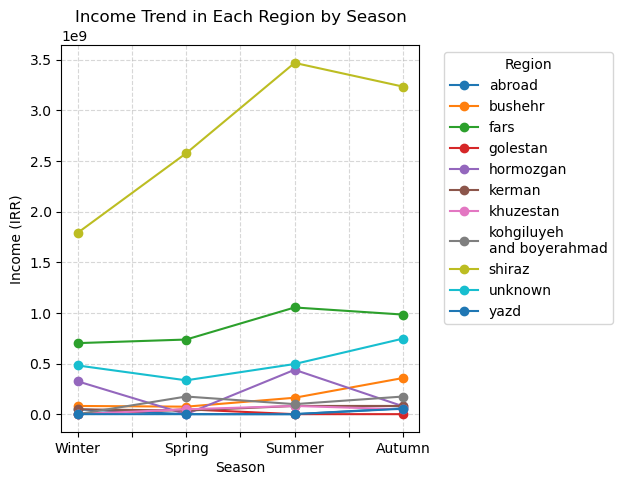
\includegraphics[width=1\textwidth]{Income Trend in Each Region by Season.png}
    \caption{Income Trend in Each Region by Season}
    \label{fig:income-region-season}
\end{figure}

\section*{3. Trend of Average Price and Total Income by Season}
Figure~\ref{fig:price-income-season} presents the seasonal patterns in pricing and revenue. Total income (bar chart) peaks in Summer, closely followed by Autumn. The average price per course (line chart) was highest in Winter (about 59 million IRR), and lowest in Spring, despite Spring having higher revenue than Winter. The decline in price from Winter to Spring, followed by a rebound, suggests strategic pricing or course mix changes influencing revenue performance.

\begin{figure}[h!]
    \centering
    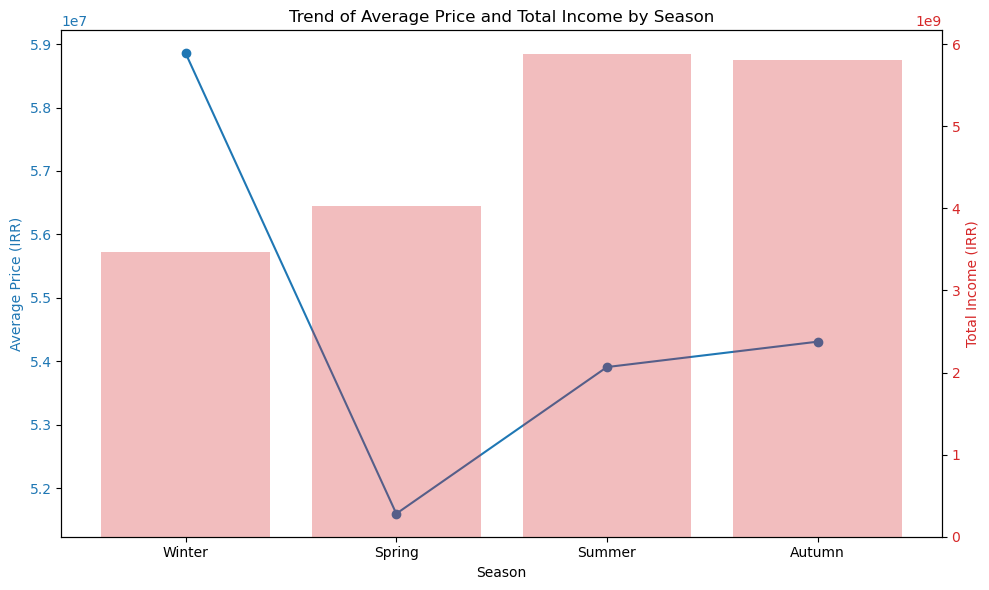
\includegraphics[width=1\textwidth]{Trend of Average Price and Total Income by Season.png}
    \caption{Trend of Average Price and Total Income by Season}
    \label{fig:price-income-season}
\end{figure}

\section*{Summary}
Summer emerges as the most active season in terms of both student volume and total income. Shiraz and Fars continue to dominate both in student count and revenue. The average price does not directly correlate with income trends, implying that volume rather than pricing is the main driver of seasonal revenue. These seasonal insights are critical for scheduling, marketing, and pricing strategy planning.

\end{document}